% Appendices
\begin{apendicesenv}

    \partapendices
    
    \chapter{Discussions on verticalization}
    \label{appendix:verticalization}
    
    Assuming buildings are parallelepipeds, i.e. all floors have the same footage, it is possible to draw geometric relationships in which the occupied area is the surface that represents the base of the parallelepiped, the number of floors its height and the built area its volume (Figure \ref{fig:desenho}). In this sense, the relationships presented in Equation \ref{eq:pavimentos}, which presents different ways of calculating verticalization, become clearer. In the equation, AC represents the built-up area; AO, the occupied area; AT, the land area; FAR the utilization coefficient and tx\_occupacao, the percentage of the land area that is occupied. Using the procedure presented, in regions with the same FAR, the lower the land occupation rate, the greater the verticalization. Similarly, for two plots with the same land occupation, the higher the FAR, the greater the verticalization.
    
    \begin{figure}[h]
        \centering
        \caption{Representation of the building as a parallelepiped}
        \includegraphics[width = \linewidth]{figuras/desenho.pdf}
        \label{fig:desenho}
    \end{figure}
    
    \begin{equation}
        \text{Pavimentos}=\frac{\text{AC}}{\text{AO}}=\frac{\text{AC}}{\text{AT}\cdot\underbrace{\frac{\text{AO}}{\text{AT}}}_\text{tx\_ocup}}=\frac{\text{AC}}{\text{AT}}\div\frac{\text{AO}}{\text{AT}}=\frac{\text{FAR}}{\text{tx\_ocup}}
        \label{eq:pavimentos}
    \end{equation}
        
    In this way, the number of floors will never be greater than the FAR, since the occupancy rate is always a number that varies between zero and one. Figure \ref{fig:ca-vert} shows the relationship between the two variables on plots in the city of São Paulo. For very small plots, the two measures are generally the same, since 100\% of the land area is usually occupied. As verticalization increases, it can be seen that FAR does not keep up with this growth, which indicates that there is a drop in the occupancy rate.
    
    \begin{figure}[h]
        \centering
        \caption{Relation between building density and verticalization in São Paulo}
        \includegraphics[width = \textwidth]{figuras/ca_vs_verticalizacao.pdf}
        \label{fig:ca-vert}
    \end{figure}
    
    \chapter{Geographic data matching methodology}
    \label{appendix:cross-referencing}
    
    To combine data that is at different geographic observation levels, you need to make a geographic \textit{join}. This makes it possible to identify all the geometries that intersect and choose a level to aggregate them. The procedure decided upon in this research was to weight the percentage of intersection, given the need to guarantee the accuracy of the data.
    
    \begin{figure}[h]
        \centering
        \caption{Parcel cutting example}
        \includegraphics[width = .75\linewidth]{figuras/corte_lote.pdf}
        \label{fig:corte-lote}
    \end{figure}
    
    Figure \ref{fig:corte-lote} shows a case of the methodology being implemented. In the example, the census sectors are represented in gray with a black outline and the plots in blue and red with dashed lines. The aim in this example is to aggregate the data at the census tract level. This way, when a plot is present in more than one census tract, it is highlighted in red and the proportion of its area that is in each census tract is calculated.
    
    From this, it is possible to distribute its attributes in a weighted manner in each census sector. If a plot has been divided in half, for example, half of its housing units, built-up area, plot area, etc. are allocated to one sector, and the other half to the other. This procedure is imprecise, but with the granularity of the data available it is the best that can be done. Another possible approach would be to calculate the centroid of the plots and assign them according to which census sector they fall into, but the bias in this case would be even greater.
    
    When the city is cut into a \textit{raster}, in Section \ref{sec:perg1}, the same procedure is carried out, but the geographical \textit{join} is made both between the lots and the \textit{raster}, and between the census tracts and the \textit{raster}. In this way, both are at the same level of observation, ensuring the least possible bias with the available data. The result of this approach can be seen in Figure \ref{fig:rasters}.
    
    \begin{figure}[h]
        \centering
        \caption{Result of cross-referencing data from \textit{raster}}
        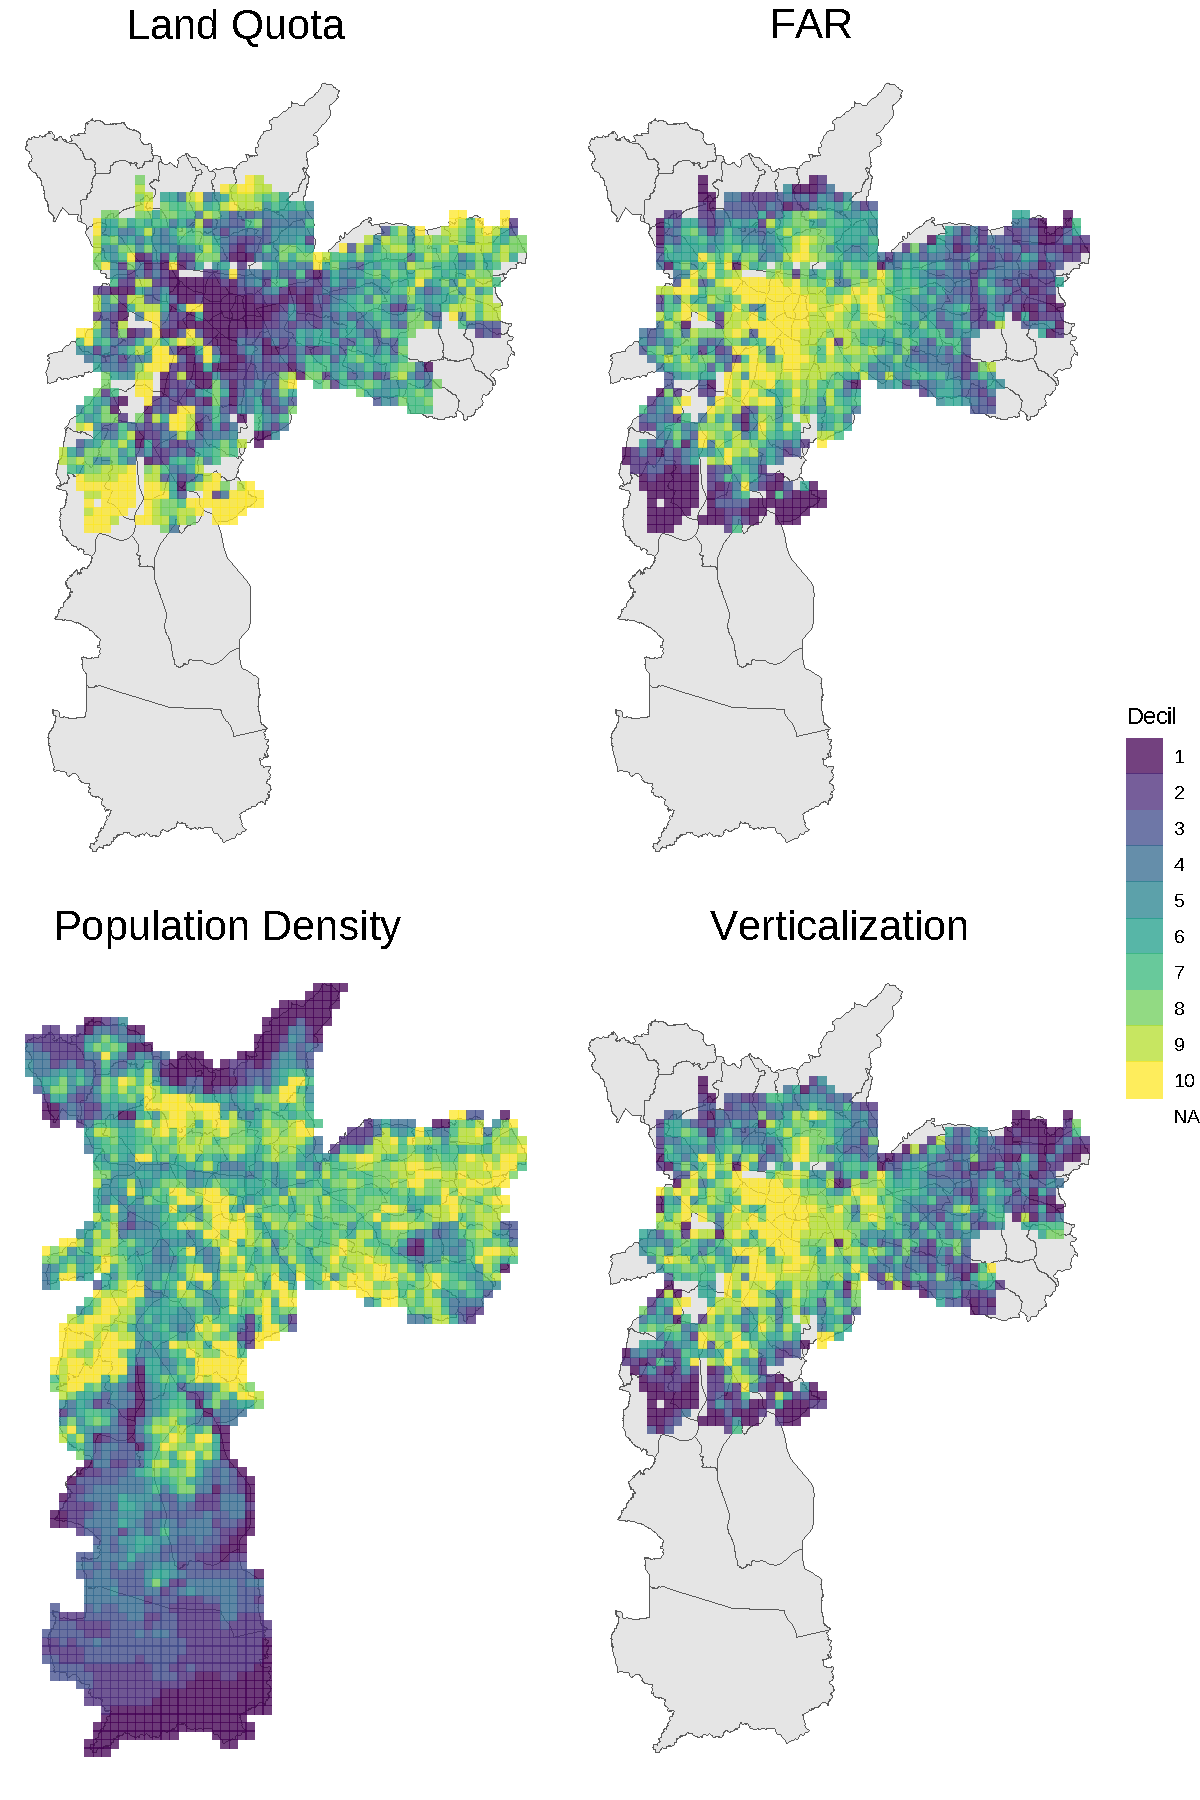
\includegraphics[width = .75\linewidth]{figuras/rasters.pdf}
        \label{fig:rasters}
    \end{figure}
    
    
    \chapter{Discussions on informality}
    \label{appendix:informality}
    
    In order to identify regions of informal housing, it is essential to compare the databases to assess the consistency of the information. The only comparable variable between the databases is the number of housing units, defined as "units" in the IPTU data and as "households" in the Census, although these categories have slightly different definitions. The disparity between the number of households in the Census and the number of units in the IPTU may suggest the presence of irregular housing. Therefore, an "irregularity index" was created, obtained from the ratio between the number of units and the sum of units and households. When this index is close to 50\%, the bases are consistent, indicating that the number of units in the IPTU is similar to the number of households in the Census. As the index approaches 0\%, there is an indication that the number of households in the Census is higher than the number of units in the IPTU, pointing to possible concentrations of informal housing.
    
    \begin{itemize}
        \item Definition of households
        
        \begin{quote}
            ``Domicile is the structurally separate and independent place that is intended to serve as a dwelling for one or more persons, or that is being used as such. Separation is characterized when the dwelling place is limited by walls or fences and covered by a roof, allowing one or more people who live there to isolate themselves from the others, for the purpose of sleeping, preparing and/or consuming their food and protecting themselves from the environment, bearing all or part of their food or living expenses. Independence is characterized when the dwelling place has direct access, allowing its residents to enter and leave without having to pass through other people's dwelling places'' \cite{IBGE2013}.
        \end{quote}
    
        \item Unit definition
        
        In the IPTU, each IPTU taxpayer is considered to represent a unit. According to the definition presented together with the data on the GeoSampa portal, ``Each urban property will correspond to an inscription number in the Tax Real Estate Registry, with real estate being understood as: I - the area of land, built or not, defined in the registration of the competent Real Estate Registry Service or in transcripts still in force''.
    \end{itemize}
    
    
    It can be seen that the peripheral census tracts have the highest irregularity rates, as evidenced by the red tones in Figure \ref{fig:balanco-raster}, indicating a significant discrepancy between the Census and IPTU databases. This pattern suggests a concentration of informal housing in these areas, where the number of households captured by the Census is substantially higher than the number of units registered with the IPTU. This behavior is not observed in the central areas of the city, where the consistency between the bases is greater, reflecting a lower prevalence of informal housing. This irregularity index therefore offers an analytical tool for spatially identifying regions with a potential presence of irregular allotments and slums, revealing the geographical distribution of informal housing in São Paulo.
    
    \begin{figure}[h]
        \caption{Geographic pattern of irregularity in São Paulo}
        \centering
        \includegraphics[width = .8\linewidth]{figuras/balanco_raster.pdf}
        \label{fig:balanco-raster}
    \end{figure}
    
    \begin{table}[h]
\caption{\textit{raster} cells with the most population density}
\centering
\fontsize{9.8pt}{11.7pt}\selectfont
\begin{tabular*}{.975\linewidth}{@{\extracolsep{\fill}}lrrrrr}
\toprule
 & \multicolumn{4}{c}{Favelas} &  \\ 
\cmidrule(lr){2-5}
Variable & 1. Paraisópolis & 2. Heliópolis  & 4. Paraisópolis & 5. Heliópolis & 3. Sé (Bela Vista) \\ 
\midrule\addlinespace[2.5pt]
Population & 29.598 & 25.280 & 23.824 & 22.920 & 24.576 \\ 
Dwellings (Censo) & 11.655 & 10.178 & 9.361 & 9.001 & 17.875 \\ 
Dwellings Occupied & 10.791 & 9.269 & 8.810 & 8.274 & 13.732 \\ 
Dwellings (IPTU) & 0 & 1.857 & 7 & 3 & 21.057 \\ 
Irregularity Spectrum & 0.00\% & 15.43\% & 0.08\% & 0.03\% & 54.09\% \\ 
Population Density & 46.247 & 39.500 & 37.225 & 35.813 & 38.400 \\ 
Area & 640.000 & 640.000 & 640.000 & 640.000 & 640.000 \\ 
\bottomrule
\label{tab:top5}

\end{tabular*}
\end{table}


    
    Table \ref{tab:top5} shows the 5 \textit{raster} cells with the highest population density. It's interesting to note that 4 of the 5 densest cells in the city are slum areas and almost entirely full of homes that are not registered with the IPTU. The overall population density of the municipality of São Paulo is 7,529 inhabitants per square kilometer, which means that this \textit{raster} cell positioned in the Paraisópolis region has a density almost four times higher than the rest of the city. Another interesting factor is the higher number of IPTU units in the Sé region, when compared to households in the census. This is one of the few regions where the irregularity spectrum exceeds 50\%. This may be associated with the high abandonment rate, which makes it difficult for interviewers to measure - the Census data indicates that 34.8\% of the households in this \textit{raster} cell are unoccupied.
    
    \chapter{Verticalization and densification in São Paulo neighborhoods}
    \label{appendix:neighborhoods}
    
    \begin{figure}[!h]
        \centering
        \caption{Population density of building patterns in São Paulo neighborhoods}
        \includegraphics[width = \linewidth]{figuras/bairros.pdf}
        \label{fig:bairros}
    \end{figure}
    
    
    The analyses in Figures \ref{fig:bairros} and \ref{fig:bairros-mapa} highlight the disparities between verticalization and population density in São Paulo's neighborhoods. In the first case, neighborhoods such as Jardim Paulista, Moema and Pinheiros exemplify highly vertical regions that, paradoxically, do not have a high population density. On the other hand, peripheral neighbourhoods like Capão Redondo have a high population density but low verticalization, reflecting a pattern of horizontal occupation and intense densification. In Figure \ref{fig:bairros}, 40 of the 96 districts were selected that have the irregularity spectrum closest to 50\%, i.e. the Census and IPTU data are similar. The special thing about these neighborhoods is that the IPTU data is more reliable.
    
    In Figure \ref{fig:bairros-mapa}, you can see on a map where the neighborhoods are where the difference between the ranking of population density and verticalization is greatest. In the red neighborhoods, where this gap is very large, there is verticalization without densification. In Figure \ref{fig:bairros-mapa-CP}, the same map is created, but to check in which regions the quota share is not translated into population density. As household density is the most important factor in defining population density, there are few cases in which the position in the ranking differs, and when it does, it is only a few positions. Even so, in the red neighborhoods fewer people live in each home, which may be associated with the strong presence of studio apartments, while the blue ones point to regions where homes are occupied by larger family groups.
    
    \begin{figure}[!h]
        \centering
        \caption{Difference between the position of population density and verticalization in the ranking of neighborhoods}
        \includegraphics[width = \linewidth]{figuras/bairros-mapa.pdf}
        \label{fig:bairros-mapa}
    \end{figure}
    
    \begin{figure}[!h]
        \centering
        \caption{Difference between the position of population density and housing density in the ranking of neighborhoods}
        \includegraphics[width = \linewidth]{figuras/bairros-mapa-cotaparte.pdf}
        \label{fig:bairros-mapa-CP}
    \end{figure}
    
    
    
    
    
    \chapter{Robustness of results}
    \label{appendix:robustness}
    
    \begin{figure}[!h]
        \centering
        \caption{Robustness of regression results for different irregularity spectra}
        \includegraphics[width = \linewidth]{figuras/robustez-regressao1pop.pdf}
        \label{fig:robustez-reg1}
    \end{figure}
    
    
    \begin{figure}[!h]
        \centering
        \caption{Robustness of DiD results for different proximity cut-offs in IPTU analysis}
        \includegraphics[width = \linewidth]{figuras/did-IPTU-bandas.pdf}
        \label{fig:robustez-did-IPTU}
    \end{figure}
    
    \begin{figure}[!h]
        \centering
        \caption{Robustness of DiD results for different proximity cut-offs in the Census analysis. (Table \ref{tab:did-censo}, column B and D)}
        \includegraphics[width = \linewidth]{figuras/did-censo-bandas.pdf}
        \label{fig:robustez-did-censo}
    \end{figure}
    
    
    
    
    
    
    
    
    
    
    
    
    
    
    
    \chapter{Other figures and tables}
    \label{appendix:figures}
    
    \clearpage
    
    \begin{figure}[h]
        \centering
        \caption{Variation over time of residential construction patterns observed in São Paulo}
        \includegraphics[width = .75\linewidth]{figuras/indicadores_tempo.pdf}
        \label{fig:indicadores-tempo}
    \end{figure}
    
    By analyzing the construction patterns over time in Figure \ref{fig:indicadores-tempo}, the densification trajectory is evident. In the figure, each line represents a quantile of the IPTU lots. By ordering the buildings in 2020 in ascending order of observed FAR, the development in position 80\% of this row has an observed FAR of 3.8. This same procedure in the year 2000 would return a development with an observed AC of 1.46. Similarly, the observed floor area, which in 2020 had a quantile of 20\% of a mere 21.7 square meters, would have had 100 square meters in 2000. This shows that in recent years São Paulo has undergone a strong densification process.
    
    
    \clearpage
    
    \begin{figure}
        \centering
        \caption{Built-up area in the municipality of São Paulo by type and use pattern}
        \includegraphics[width = .8\linewidth]{figuras/tree_area_construida.pdf}
        \label{fig:area_construida}
    \end{figure}
    
    Figure \ref{fig:area_construida} shows the distribution of the built-up area by type and standard of use. In São Paulo, 70\% of the built area is residential, and the most common residential standard is "C". The standard is a division made in the calculation of the IPTU \cite{lei10235_1986}, to create tax discounts for properties with desirable characteristics from the point of view of urban planning, such as greater densification, or for properties owned by people with lower purchasing power. Measurements such as footage, ceiling height, parking space, number of floors, architectural elements, building materials, etc. are all factors taken into account to determine the standard. In the case of "C", it is in the middle of the density scale, with "A" being the densest and "E" the least. The second most common use is commercial, followed by industrial and entertainment. The entertainment category includes religious temples, clubs, sports stadiums, cinemas, airports, museums and zoos, among others.
    
    
    
    
    
    
    \begin{figure}[!h]
        \centering
        \caption{Axis regions (painted in blue)}
        \includegraphics[width = .85\linewidth]{figuras/macroareas-eixos.pdf}
        \label{fig:eixos}
    \end{figure}
    
    \clearpage
    
    \begin{figure}[!h]
        \centering
        \caption{Distribution of the number of residents in each cell of the raster}
        \includegraphics[width = .85\linewidth]{figuras/populacao-distribuicao-raster.pdf}
        \label{fig:populacao-rasters}
    \end{figure}
    
    
    
    
    
    
    \end{apendicesenv}
        
        